\documentclass[a4paper]{ctexart}
\usepackage{ctex}
\usepackage{times}
\usepackage{setspace}
\usepackage{fancyhdr}
\usepackage{graphicx}
\usepackage{wrapfig}
\usepackage{array}
\usepackage{fontspec,xunicode,xltxtra}
\usepackage{titlesec}
\usepackage{titletoc}
\usepackage[titletoc]{appendix}
\usepackage[top=30mm,bottom=30mm,left=20mm,right=20mm]{geometry}
\usepackage{enumerate}
\usepackage{caption}
\usepackage{abstract}
\usepackage{amsmath}
\setmainfont{TeX Gyre Pagella}

\captionsetup[figure]{name={图},labelsep=period,font={bf,small}}

%---------------------------------------------------------------------
%	页眉页脚设置
%---------------------------------------------------------------------
\fancypagestyle{plain}{\pagestyle{fancy}}%改变章节首页页眉
\pagestyle{fancy}
\lhead{\kaishu~无线射频识别技术课程作业~}
\rhead{\kaishu~纪港~尹达恒~郭星宇~孙硕~孙瑜博~王雷}
\cfoot{\thepage}

%---------------------------------------------------------------------
%	目录页设置
%---------------------------------------------------------------------
\titlecontents{section}[2em]{\vspace{0.1\baselineskip}\songti\zihao{-4}}{\thecontentslabel\ }{}
{\hspace{.5em}\titlerule*[4pt]{$\cdot$}\contentspage}
\titlecontents{subsection}[4em]{\vspace{0.1\baselineskip}\songti\zihao{-4}}{\thecontentslabel\ }{}
{\hspace{.5em}\titlerule*[4pt]{$\cdot$}\contentspage}

\ctexset {
	section = {
		number = \arabic{section},
		format = \Large\bfseries,
	},
	subsection = {
		number = \arabic{section}.\arabic{subsection},
	}
}

\begin{document}
%---------------------------------------------------------------------
%	封面设置
%---------------------------------------------------------------------
\begin{titlepage}
	\begin{center}
    
\includegraphics[width=0.9\textwidth]{figure//Njust.png}\\
    \vspace{10mm}
    \textbf{\zihao{2}\kaishu{物联网工程学院}}\\[0.8cm]
    \textbf{\zihao{2}\kaishu{无线射频识别技术课程作业}}\\[3cm]
    \textbf{\zihao{2}\kaishu{RFID技术基本原理与日常应用}}\\[3cm]
	\vspace{\fill}
	\setlength{\extrarowheight}{3mm}
	{\songti\zihao{3}	
		\begin{tabular}{rl}
			{\makebox[4\ccwd][s]{班\qquad 级:}}& ~\kaishu 物联1601\\
			{\makebox[4\ccwd][s]{组\qquad 长:}}& ~\kaishu 纪港 \\
			{\makebox[4\ccwd][s]{组\qquad 员:}}& ~\kaishu 尹达恒、郭星宇、孙硕、孙瑜博、王雷 \\
			{\makebox[4\ccwd][s]{指导老师:}} & ~\kaishu 孙子文\\
		\end{tabular}
	}\\[2cm]
	\vspace{\fill}
	\zihao{4}
	2018\textasciitilde 2019第二学期\\
	\today
	\end{center}	
\end{titlepage}



%---------------------------------------------------------------------
%  目录页
%---------------------------------------------------------------------
\tableofcontents % 生成目录
\newpage
%---------------------------------------------------------------------
%  实验一
%---------------------------------------------------------------------
\begin{spacing}{1.5}
\songti\zihao{-4}
\section{RFID通信技术简介}
RFID是一种通信技术,可通过无线电信号识别特定目标并读写相关数据,而无需识别系统与特定目标之间建立机械或光学接触。它不仅可以实现对被识别物体的自动识别与快速读写,还可以同时识别多个标签以及高速移动的标签,操作快捷简单,能工作于各类不同的恶劣环境中,是目前最准确、适应性最强的自动识别技术。

\section{RFID通信技术原理}
目前,RFID技术还未出台全球的统一标准,每个国家的标准都不一样,导致全球多种标准并存的局面。但随着RFID在全球物流行业的大规模应用,ISO制定的一些RFID国际标准已经得到全球各个业界的广泛认可。本文使用无源的RFID电子标签,支持ISOI8000—6C(EPCGEN2)国际标准协议,工作频率在860~960MHz之间,不同的工作频率需设计不同的天线,下面主要介绍RFID的天线设计及其应用。

RFID技术中最难的部分是天线的设计,天线面积越大并不代表其感应强度越大,为了获得最佳的测量效果,必须知道设备的大小,然后才能确定天线的大小。天线是一敏感的物体,制作天线采用的电阻、电容、电感等元件必须具有较高的精度,否则天线制作就可能失败。天线的等效电路如图\ref{circ}所示。

\begin{figure}[htbp]
	\centering
	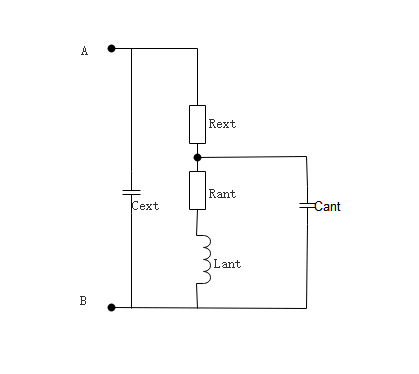
\includegraphics [width=0.8\textwidth]{figure//circ.png}
	\caption{RFID标签天线等效电路图}\label{circ}
\end{figure}

天线的性能主要与天线电阻$R_{ant}$和天线电感$L_{ant}$的大小有关。天线电容$C_{ant}$和天线电阻$R_{ant}$的大小与天线线圈的大小有关,可以用仪器直接测量。当计算天线的品质因数$Q$和天线调谐时线圈的电容$C_{ant}$可以忽略。天线的几个重要参数估算公式如下所示:
\begin{equation}
\begin{split}
L_{ant}&=2L_{1}N_{1}^{18}[ln(\frac{L_{1}}{D_{1}})-K],\\
Q&=\frac{\omega_{R}L_{ant}}{R_{ant}},\\
R_{ext}&=\frac{\omega_{R}L_{ant}}{Q}-R_{ant},\\
C_{ext}&=\frac{R_{ant}^{2}+(\omega_{R}L_{ant}-1/\omega_{R}C_{ant})^{2}}{\frac{\omega_{R}L_{ant}}{C_{ant}}(1/\omega_{R}C_{ant}-\omega_{R}L_{ant})-\frac{R_{ant}^{2}}{C_{ant}^{2}}}
\end{split}
\end{equation}

其中:$L_{1}$为一圈(匝)导线环的长度;$D_{1}$为线圈的直径或导体的宽度;$N_{1}$为线圈的匝数;$K$为天线的系数(环形为1.07,方形为1.47);$\omega_{R}=2\pi f_{R}$,$f_{R}$为RFID工作频率,由于RFID可以工作在860~960MHz之间,与国内手机GSM900应用会有冲突,所以使用时一般只采用860~870MHz作为RFID工作频率范围。

\section{RFID识别系统组成与功能}
RFID识别系统通常由前端的射频终端和后台的计算机信息管理系统构成。射频终端一般由读写器和标签组成,标签用来标识存储物品的各种属性信息;读写器用来进行信息采集,利用射频信号对标签进行识别并与计算机信息系统进行通信。

\section{RFID识别系统基本原理}
\subsection{电子标签}
RFID电子标签由耦合元件与芯片组成,含有微处理器、E2PROM及收发电路,储存着产品的详细信息。每一个产品的电子标签都是唯一的,含有加密逻辑,无法修改和仿造。

\subsection{读写器}
RFID读写器通过天线发射出一定频率的射频信号,当电子标签进入读写器的工作范围内,由于电磁感应,其天线会产生感应电流,使得电子标签获得能量被激活,从而向读写器发送自身储存的编码信息。读写器将收到的信息进行解码送至后台计算机信息管理系统,使得计算机能根据逻辑运算判断标签的合法性,针对不同的设定做出相应的处理与控制。

\subsection{后台计算机信息管理系统}
计算机信息管理系统对从前端的射频终端发来的标签信息进行接收与存储,并通过Internet与其他管理系统进行联网,搭起信息平台,通过信息平台能够监管和查询产品的流向。

\section{RFID识别系统应用领域}
\subsection{高速公路收费及智能交通系统}
高速公路自动收费系统是射频识别技术最成功的应用之一。目前中国的高速公路发展非常快,地区经济发展的先决条件就是有便利的交通条件,而高速公路收费却存在一些问题,一是交通堵塞,在收费站口,许多车辆要停车排队交费,成为交通瓶颈问题;二是少数不法的收费员贪污收取的过路费,使国家蒙受了财政收入损失。RFID技术应用在高速公路自动收费上能够充分体现该技术的优势。在车辆高速通过收费站的同时自动完成缴费,解决了交通的瓶颈问题,提高了车行速度,避免了拥堵,提高了收费计算效率,同时可以解决收费员贪污收取的过路费的问题。

\subsection{生产的自动化及过程控制}
RFID技术因其具有抗恶劣环境能力强、非接触识别等特点,在生产过程控制中有很多应用。通过在大型工厂的自动化流水作业线上使用RFID技术,实现了物料跟踪和生产过程自动控制、监视,提高了生产效率,改进了生产方式,降低了成本。在生产线的自动化及过程控制方面,德国BMW公司为保证汽车在流水线各位置准确地完成装配任务,将RFID系统应用在汽车装配线上。而Motorola公司则采用了RFID技术的自动识别工序控制系统,满足了半导体生产对环境的特殊要求,同时提高了生产效率。

\subsection{车辆的自动识别以及防盗}
通过建立采用射频识别技术的自动车号识别系统,能够随时了解车辆的运行情况,不仅实现了车辆的自动跟踪管理,还可以大大减少发生事故的可能性,并且可以通过射频识别技术对车辆的主人进行有效验证,防止车辆偷盗发生,在车辆丢失以后可以有效寻找丢失的车辆。采用射频识别技术可以对道路交通流量进行实时监控、统计、调度,还可以用作车辆闯红灯记录报警,被盗(可疑)车辆报警与跟踪,特殊车辆跟踪,肇事逃逸车辆排查等。据报道,英国计划在汽车上安装射频芯片,行驶超速时将被自动“举报”。

\subsection{电子票证}
使用电子标签来代替各种“卡”,实现非现金结算,解决了现金交易不方便也不安全以及以往的各种磁卡、IC卡容易损坏等问题。同时电子标签用起来方便、快捷,还可以同时识别几张电子标签,并行收费。射频识别系统,特别是非接触IC卡(电子标签)应用潜力最大的领域之一就是公共交通领域。用电子标签作为电子车票,具有使用方便、可以缩短交易时间、降低运营成本等优势。1996年1月韩国在首尔的600辆公共汽车上安装射频识别系统用于电子月票,实现了非现金结算,方便了市民出行。而德国汉莎航空公司则开始试用射频卡(电子标签)作为飞机票,改变了传统的机票购销方式,简化了机场入关手续。

\subsection{货物跟踪管理及监控}
射频识别技术为货物的跟踪管理及监控提供了方便、快捷、准确的自动化技术手段。以射频识别技术为核心的集装箱自动识别,成为全球范围内最大的货物跟踪管理应用。将记录有集装箱位置、物品类别、数量等数据的电子标签安装在集装箱上,借助射频识别技术,就可以确定集装箱在货场内的确切位置。系统还可以识别未被允许的集装箱移动,有利于管理和安全。在货物的跟踪、管理及监控方面,澳大利亚和英国的希斯罗机场将射频识别技术应用于旅客行李管理中,大大提高了分拣效率,降低了出错率。在几年前,欧共体就要求从1997年开始生产的新车型必须具有基于射频识别技术的防盗系统。目前我国铁路部门也计划推广行包自动追踪管理系统,但真正应用还要假以时日。

\subsection{仓储、配送等物流环节}
将射频识别系统用于智能仓库货物管理,可以有效地解决仓库里与货物流动相关的信息的管理,监控货物信息,实时了解库存情况,自动识别货物,确定货物的位置。

\subsection{邮件、邮包的自动分拣系统}
射频识别技术已经被成功应用到邮政领域的邮包自动分拣系统中,该系统具有非接触、非视线数据传输的特点,所以包裹传送中可以不考虑包裹的方向性问题。另外,当多个目标同时进入识别区域时,可以同时识别,大大提高了货物分拣能力和处理速度。另外,由于电子标签可以记录包裹的所有特征数据,更有利于提高邮包分拣的准确性。

\subsection{动物跟踪和管理}
射频识别技术可以用于动物跟踪与管理。将用小玻璃封装的电子标签植于动物皮下,可以标识牲畜,监测动物健康状况等重要信息,为牧场的管理现代化提供了可靠的技术手段。在大型养殖场,可以通过采用射频识别技术建立饲养档案、预防接种档案等,达到高效、自动化管理牲畜的目的,同时为食品安全提供保障。在动物的跟踪及管理方面,许多发达国家采用射频识别技术,通过对牲畜个体识别,保证牲畜大规模疾病爆发期间对感染者的有效跟踪及对未感染者进行隔离控制。

\subsection{门禁保安}
未来的门禁保安系统都可以应用电子标签,一卡可以多用,比如做工作证、出入证、停车证、饭店住宿证甚至旅游护照等。使用电子标签可以有效地识别人员身份,进行安全管理以及高效收费,简化了出入手续,提高了工作效率,并且有效地进行了安全保护。人员出入时该系统会自动识别身份,非法闯入时会有报警。安全级别要求高的地方,还可以结合其他的识别方式,将指纹、掌纹或颜面特征存入电子标签。

\subsection{防伪}
伪造问题在世界各地都是令人头疼的问题,现在应用的防伪技术如全息防伪等同样会被不法分子伪造。将射频识别技术应用在防伪领域有它自身的技术优势,它具有成本低而又很难伪造的优点。电子标签的成本相对便宜,且芯片的制造需要有昂贵的工厂,使伪造者望而却步。电子标签本身具有内存,可以储存、修改与产品有关的数据,利于进行真伪的鉴别。利用这种技术不用改变现行的数据管理体制,唯一的产品标识号完全可以做到与已用数据库体系兼容。

\section{生活中的RFID典型应用:疫苗追踪}
以我国目前医药物流的发展现状来说,每支疫苗都使用RFID标签进行标识,实现疫苗的追踪,还是不太可能。现在大多是将二维条码与RFID标签联合使用,用二维条码来记录疫苗信息,做到每支疫苗都有唯一标识的零售包装,再应用RFID电子标签标识疫苗的生产物流包装,记录包装箱内疫苗的信息,实现疫苗的供应链追踪以及问题疫苗的追溯功能。RFID标签的应用,使得疫苗生产企业能够在每个包装箱建立唯一的EPC编码,它被认为是识别所有物件唯一有效方式,EPC编码虽只能记录有限的识别信息,但它有对应的后台数据库作为支持,能够迅速查询疫苗的各个包装信息。当疫苗出库时,贴有RFID电子标签的就会被跟踪,保证疫苗在分销过程中的物流、仓储、接种环节都能得到监控。RFID将遏制假冒伪劣疫苗的出现,防止出现疫苗流失,加快疫苗库存的周转,提高疫苗的召回速度。在物流环节中使用RFID技术,能对疫苗冷链运输过程中的存储温度、运输车辆、车辆位置及运输时间等信息进行记录,将记录的信息通过GPRS无线通信或车载有线网络与物流公司的本地数据库进行通信,就能使疫苗的生产、物流、仓储、接种四大环节环环相扣,每一个环节出现问题都能及时找出源头。
\end{spacing}
\end{document}